% -*- latex -*-
%%%%%%%%%%%%%%%%%%%%%%%%%%%%%%%%%%%%%%%%%%%%%%%%%%%%%%%%%%%%%%%%
%%%%%%%%%%%%%%%%%%%%%%%%%%%%%%%%%%%%%%%%%%%%%%%%%%%%%%%%%%%%%%%%
%%%%
%%%% This text file is part of the source of 
%%%% `Introduction to High-Performance Scientific Computing'
%%%% by Victor Eijkhout, copyright 2012-6
%%%%
%%%% This book is distributed under a Creative Commons Attribution 3.0
%%%% Unported (CC BY 3.0) license and made possible by funding from
%%%% The Saylor Foundation \url{http://www.saylor.org}.
%%%%
%%%%
%%%%%%%%%%%%%%%%%%%%%%%%%%%%%%%%%%%%%%%%%%%%%%%%%%%%%%%%%%%%%%%%
%%%%%%%%%%%%%%%%%%%%%%%%%%%%%%%%%%%%%%%%%%%%%%%%%%%%%%%%%%%%%%%%

In the discussion of \acp{IBVP} (section~\ref{sec:implicit-euler}) you
saw that implicit operations can have great advantages from the point
of numerical stability. However, you also saw that they make the
difference between methods based on a simple operation such as the
matrix-vector product, and ones based on the more complicated linear
system solution. There are further problems with implicit methods when
you start computing in parallel.

\begin{exercise}
  Let $A$ be the matrix
  \begin{equation} A=
  \begin{pmatrix}
    a_{11}&&\emptyset\\ a_{21}&a_{22}\\ &\ddots&\ddots\\ 
    \emptyset&&a_{n,n-1}&a_{nn}
  \end{pmatrix}.\label{eq:ex:bidiagonal}
  \end{equation}
  Show that the matrix vector product $y\leftarrow Ax$ and the system
  solution $x\leftarrow A\inv y$, obtained by solving the
    triangular system $Ax=y$, not by inverting~$A$, have the same
  operation count.

  Now consider parallelizing the product $y\leftarrow Ax$. Suppose we
  have $n$ processors, and each processor~$i$ stores $x_i$ and the
  $i$-th row of~$A$. Show that the product $Ax$ can be computed without
  idle time on any processor but the first.

  Can the same be done for the solution of the triangular system
  $Ax=y$? Show that the straightforward implementation has every
  processor idle for an $(n-1)/n$ fraction of the computation.
\end{exercise}

We will now see a number of ways of dealing with this inherently
sequential component.

\Level 1 {Wavefronts}
\label{sec:wavefront}
\index{wavefront|(}

Above, you saw that solving a lower triangular system of size~$N$ can
have sequential time complexity of $N$ steps. In practice, things are
often not quite that bad. Implicit algorithms such as solving a
triangular system are inherently sequential, but the number of 
steps can be less than is apparent at first.

\begin{exercise}
  Take another look at the matrix from a two-dimensional \ac{BVP} on
  the unit square,
  discretized with central differences.
  Derive the matrix structure if we
  order the unknowns by diagonals. What can you say about the sizes of
  the blocks and the structure of the blocks themselves?
\end{exercise}

Let us take another look at
figure~\ref{fig:laplacedomain} that describes the difference stencil
of a two-dimensional \ac{BVP}. The corresponding picture for the lower
triangular factor is
\begin{figure}
  \begin{quote}
    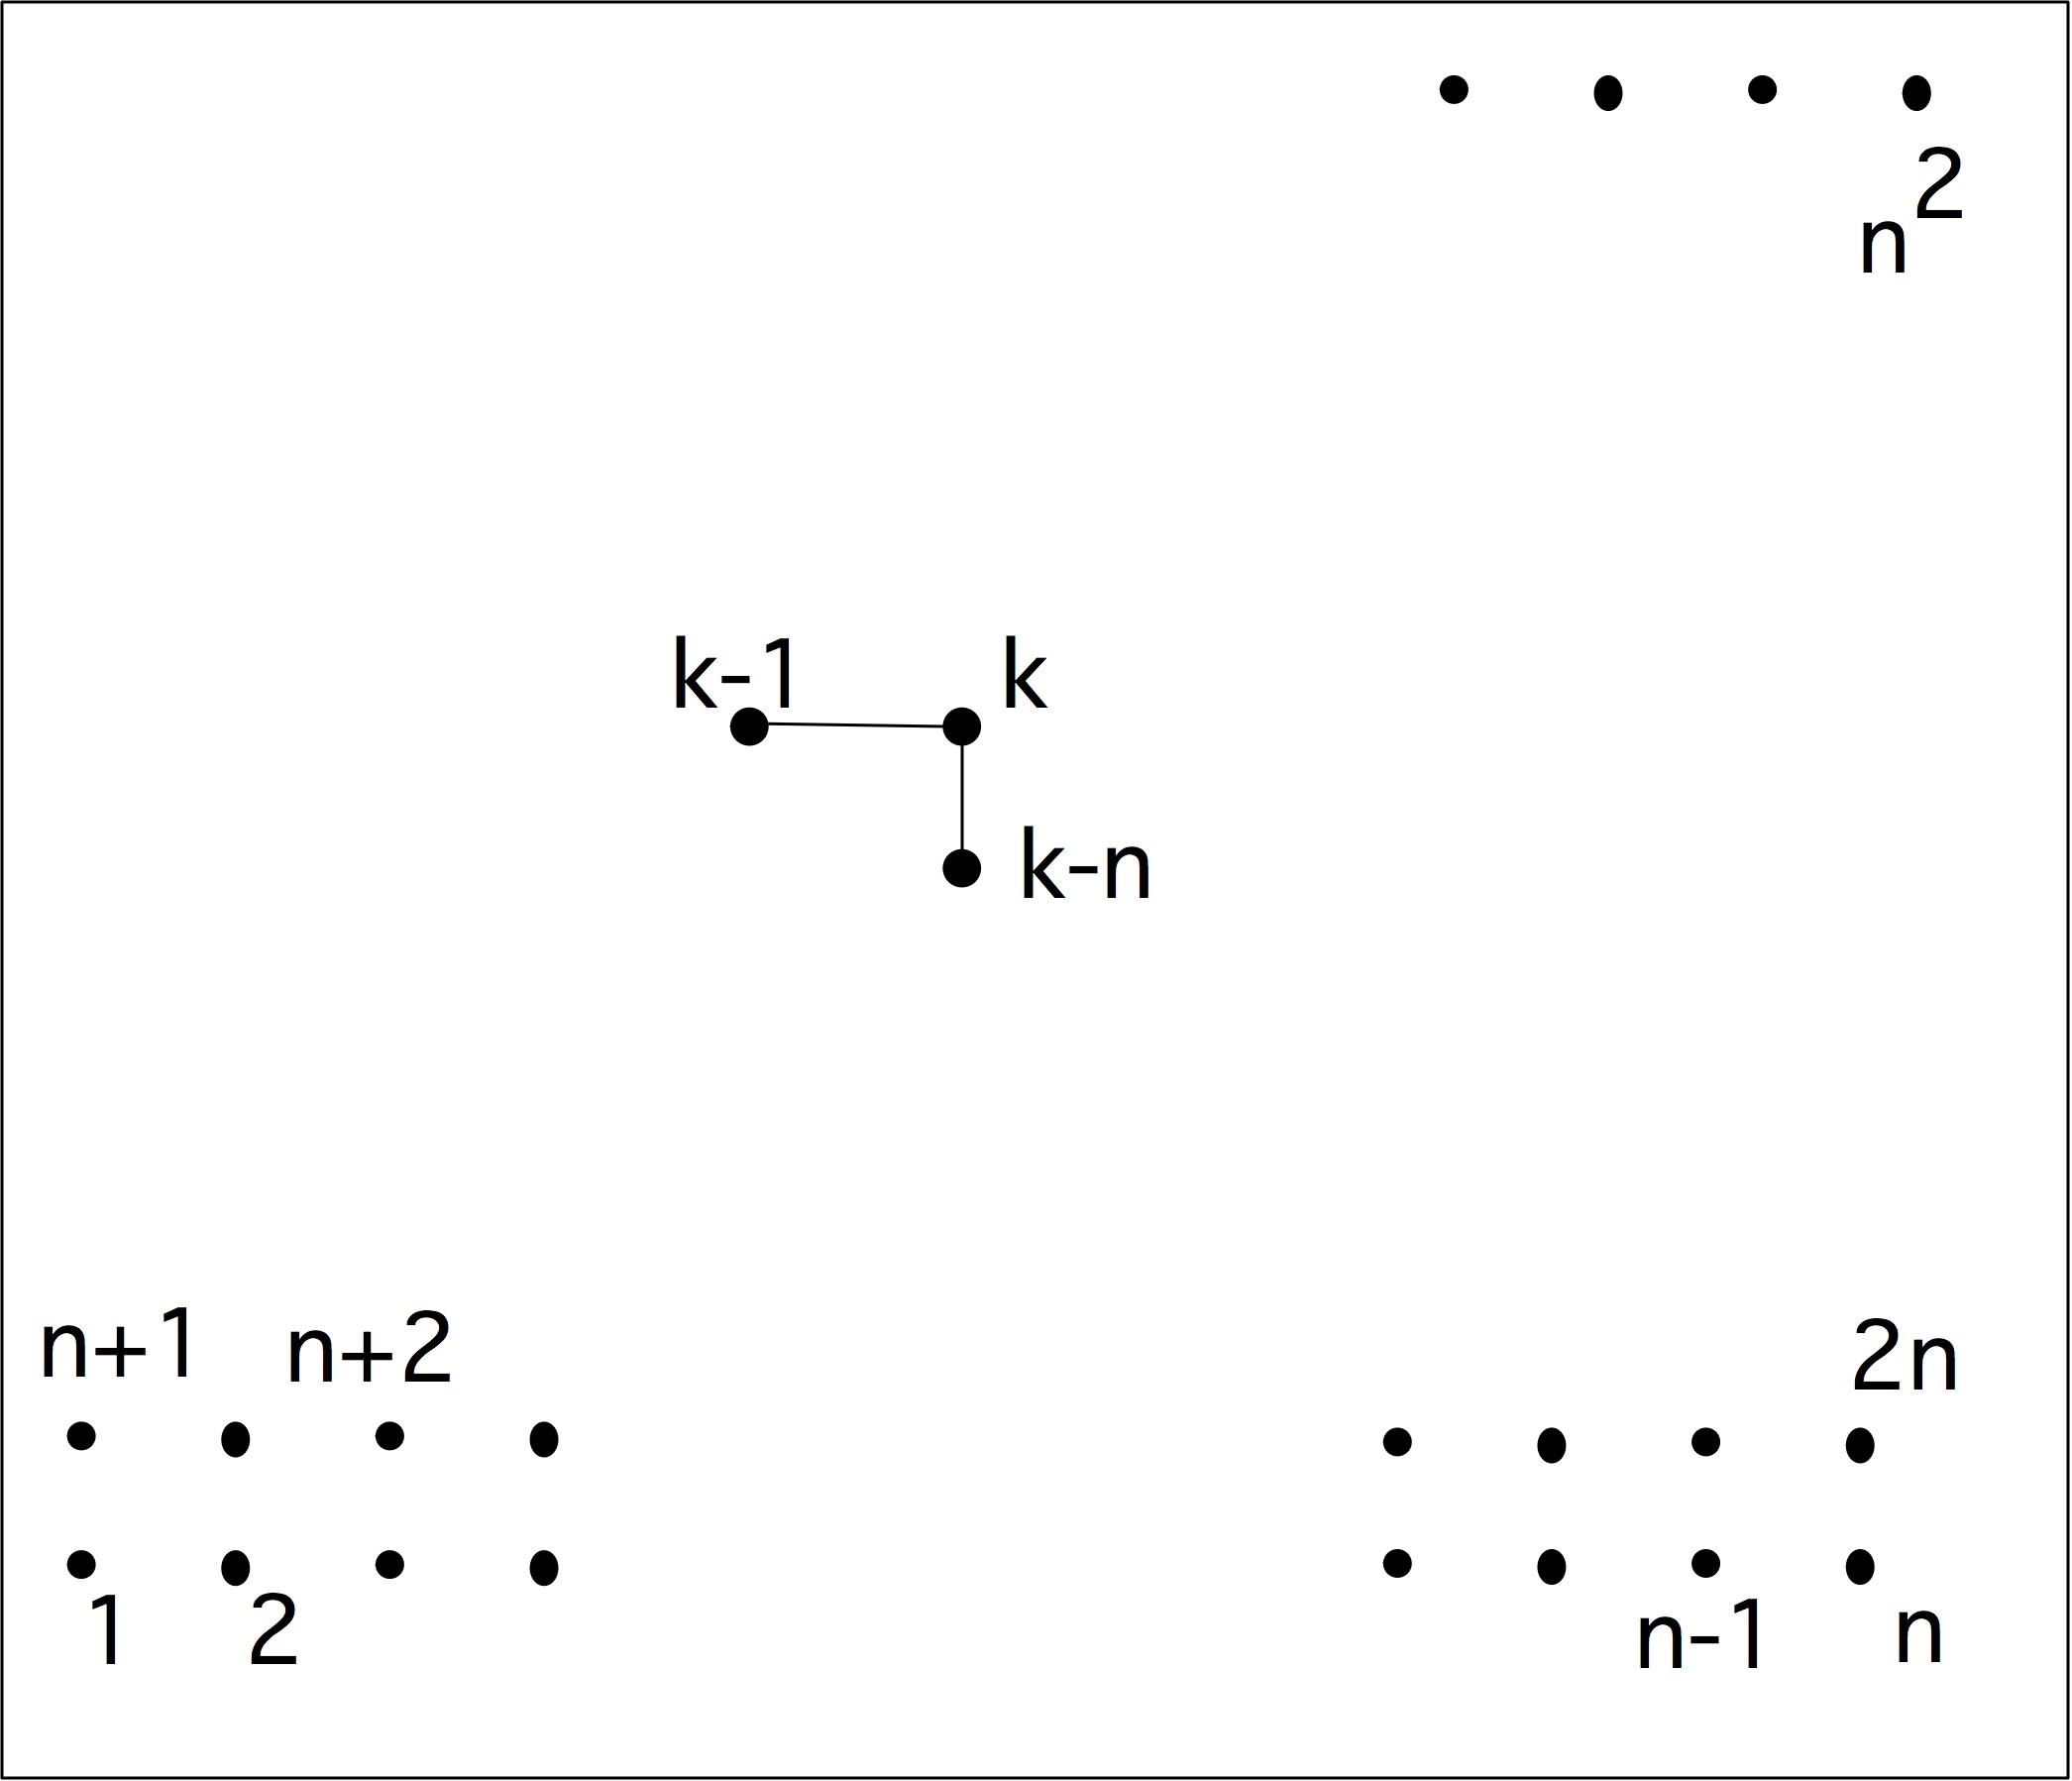
\includegraphics[scale=.12]{graphics/laplacelower}
  \end{quote}
  \caption{The difference stencil of the $L$ factor of the matrix
    of a two-dimensional \ac{BVP}}
  \label{fig:laplacelower}
\end{figure}
in figure~\ref{fig:laplacelower}. This describes the sequentiality of
the lower triangular solve process $x\leftarrow L\inv y$:
\[ x_k = y_k - \ell_{k,k-1}x_{k-1} - \ell_{k,k-n}x_{k-n} \]
In other words, the value at point~$k$ can be found if its neigbours
to the left (that is, variable $k-1$) and below (variable $k-n$) are
known. 

Turning this around, we see that, if we know $x_1$, we can not only
find $x_2$, but also $x_{n+1}$. In the next step we can determine
$x_3$, $x_{n+2}$, and $x_{2n+1}$. Continuing this way, we can solve
$x$ by \emph{wavefronts}: the values of $x$ on each wavefront are
independent, so they can be solved in parallel in the same sequential
step.

\begin{exercise}
  Finish this argument. What is the maximum number of processors we
  can employ, and what is the number of sequential steps? What is the
  resulting efficiency?
\end{exercise}

Of course you don't have to use actual parallel processing
to exploit this parallelism. Instead you could use a
\indexterm{vector processor}, \indextermbus{vector}{instructions},
or a \indexac{GPU}~\cite{Liu:cudasw2009}.

In section~\ref{sec:fill-ordering} you saw the
\indexterm{Cuthill-McKee ordering} for reducing the fill-in of a
matrix. We can modify this algorithm as follows to give wavefronts:
\begin{enumerate}
\item Take an arbitrary node, and call that `level zero'.
\item For level~$n+1$, find points connected to
  level~$n$, that are not themselves connected.
\item For the so-called `reverse Cuthill-McKee ordering', reverse the
  numbering of the levels.
\end{enumerate}
\begin{exercise}
  This algorithm is not entirely correct. What is the problem; how can
  you correct it? Show that the resulting permutated matrix is no
  longer tridiagonal, but will likely still have a band structure.
\end{exercise}
\index{wavefront|)}

\Level 1 {Recursive doubling}
\label{sec:recdouble}
\index{recursive doubling|(textbf}

One strategy for dealing with recurrences is
\emph{recursive doubling}, which you already saw in
exercise~\ref{ex:recursivedoubling}. Here we will discuss it in a more
systematic manner. First, take the matrix
from~\eqref{eq:ex:bidiagonal} and scale it to be of the form
\[ 
  \begin{pmatrix}
    1&&\emptyset\\ b_{21}&1\\ &\ddots&\ddots\\ 
    \emptyset&&b_{n,n-1}&1
  \end{pmatrix}
\]
which we write as $A=I+B$.

\begin{exercise}
  How does solving the system $(I+B)x=y$ help in solving $Ax=y$? What
  are the operation counts of solving the system in the two different ways?
\end{exercise}

Now we do something that looks like Gaussian elimination, except that
we do not start with the first row, but the second. (What would happen
if you did Gaussian elimination or LU decomposition on the matrix
$I+B$?) We use the second row to eliminate~$b_{32}$:
\[
  \begin{pmatrix}
    1&&&\emptyset\\ &1\\ &-b_{32}&1\\ &&&\ddots\\
    \emptyset&&&&1
  \end{pmatrix}\times
  \begin{pmatrix}
    1&&&\emptyset\\ b_{21}&1\\ &b_{32}&1\\ &&\ddots&\ddots\\ 
    \emptyset&&&b_{n,n-1}&1
  \end{pmatrix}
  =
  \begin{pmatrix}
    1&&&\emptyset\\ b_{21}&1\\ -b_{32}b_{21}&0&1\\ 
    \emptyset&&b_{n,n-1}&1
  \end{pmatrix}
\]
which we write as $L^{(2)}A=A^{(2)}$. We also compute
$L^{(2)}y=y^{(2)}$ so that $A^{(2)}x=y^{(2)}$ has the same solution as
$Ax=y$. Solving the transformed system gains us a little: after we
compute~$x_1$, $x_2$~and~$x_3$ can be computed in parallel.

Now we repeat this elimination process by using the fourth row to
eliminate~$b_{54}$, the sixth row to eliminate~$b_{76}$, et
cetera. The final result is, summarizing all~$L^{(i)}$ matrices:
{\small
\[
  \begin{pmatrix}
    1&&&&&&&\emptyset\\ 0&1\\ &-b_{32}&1\\ &&0&1\\
    &&&-b_{54}&1\\ &&&&0&1\\ &&&&&-b_{76}&1\\ &&&&&&\ddots&\ddots\\
  \end{pmatrix}\times (I+B) =
  \begin{pmatrix}
    1&&&&&&&\emptyset\\ b_{21}&1\\ -b_{32}b_{21}&0&1\\ 
    &&b_{43}&1\\ &&-b_{54}b_{43}&0&1\\
    &&&&b_{65}&1\\ &&&&-b_{76}b_{65}&0&1\\ &&&&&\ddots&\ddots&\ddots
  \end{pmatrix}
\]
}
which we write as $L(I+B)=C$, and solving $(I+B)x=y$ now becomes
$Cx=L\inv y$.

This final result needs close investigation.
\begin{itemize}
\item First of all, computing $y'=L\inv y$ is simple. (Work out the
  details. How much parallelism is available?)
\item Solving $Cx=y'$ is still sequential, but it no longer takes $n$
  steps: from $x_1$ we can get $x_3$, from that we get~$x_5$, et
  cetera. In other words, there is only a sequential relationship
  between the odd numbered components of~$x$.
\item The even numbered components of~$x$ do not depend on each other,
  but only on the odd components: $x_2$~follows from~$x_1$, $x_4$
  from~$x_3$, et cetera. Once the odd components have been computed,
  admittedly sequentially, this step is fully parallel.
\end{itemize}
We can describe the sequential solving of the odd components by
itself:
\[ 
  \begin{pmatrix}
    1&&\emptyset\\ c_{21}&1\\ &\ddots&\ddots\\ 
    \emptyset&&c_{n,n-1}&1
  \end{pmatrix}
  \begin{pmatrix}
    x_1\\ x_3\\ \vdots\\ x_n
  \end{pmatrix} = 
  \begin{pmatrix}
    y'_1\\ y'_3\\ \vdots\\ y'_n
  \end{pmatrix}
\]
where $c_{i+1i}=-b_{2n+1,2n}b_{2n,2n-1}$. In other words, we have
reduced a size~$n$ sequential problem to a sequential problem of the
size kind and a parallel problem, both of size~$n/2$. Now we can
repeat this procedure recursively, reducing the original problem to a
sequence of parallel operations, each half the size of the former.

The process of computing all partial sums through recursive doubling
is also referred to as a parallel 
\indexterm{prefix operation}. Here we use a prefix sum, but in the abstract it
can be applied to any associative operator.

\index{recursive doubling|)}

\Level 1 {Approximating implicit by explicit operations, series expansion}
\label{sec:implicit-becomes-explicit}

There are various reasons why it is sometimes allowed to replace an
implicit operation, which, as you saw above, can be problematic in
practice, by a different one that is practically more advantageous.
\begin{itemize}
\item Using an explicit method for the heat equation
  (section~\ref{sec:heateq}) instead of an
  implicit one is equally legitimate, as long as we observe step size
  restrictions on the explicit method.
\item Tinkering with the preconditioner
  (section~\ref{sec:nonstationary}) in an iterative method is allowed,
  since it will only affect the speed of convergence, not the solution
  the method converges to. You already saw one example of this general
  idea in the \indexterm{block Jacobi} method;
  section~\ref{sec:block-jacobi}. In the rest of this section you will
  see how recurrences in the preconditioner, which are implicit
  operations, can be replaced by explicit operations, giving various
  computational advantages.
\end{itemize}

Solving a linear system is a good example of an implicit operation,
and since this comes down to solving two triangular systems, let us
look at ways of finding a computational alternative to solving a lower
triangular system. If $U$ is upper triangular and nonsingular, we let
$D$ be the diagonal of~$U$, and we write $U=D(I-B)$ where $B$ is an
upper triangular matrix with a zero diagonal, also called a
\indextermsub{strictly upper triangular}{matrix}; we say that $I-B$ is
a \indextermsub{unit upper triangular}{matrix}.

\begin{exercise}
  Let $A=LU$ be an LU factorization where $L$ has ones on the
  diagonal. Show how solving a system $Ax=b$ can be done, involving
  only the solution of unit upper and lower triangular systems. Show
  that no divisions are needed during the system solution.
\end{exercise}

Our operation of interest is now solving the system $(I-B)x=y$. We
observe that
\begin{equation}
  (I-B)\inv = I+B+B^2+\cdots
  \label{eq:neuman-series}
\end{equation}
and $B^n=0$ where $n$ is the matrix size (check
this!), so we can solve $(I-B) x = y$ exactly by 
\[ x = \sum_{k=0}^{n-1}B^k y. \]
Of course, we want to avoid computing the powers~$B^k$ explicitly, so
we observe that
\begin{equation}
 \sum_{k=0}^1B^ky = (I+B)y,\quad \sum_{k=0}^2B^ky =
 (I+B(I+B))y,\quad \sum_{k=0}^3B^ky = (I+B(I+B((I+B))))y,
 \label{eq:horner}
\end{equation}
et cetera.
The resulting algorithm for evaluating $\sum_{k=0}^{n-1}B^k y$ is
called \indexterm{Horner's rule}, and you see that it avoids computing
matrix powers~$B^k$.

\begin{exercise}
  Suppose that $I-B$ is bidiagonal.  Show that the above calculation
  takes $n(n+1)$ operations. What is the operation count for computing
  $(I-B)x=y$ by triangular solution?
\end{exercise}

We have now turned an implicit operation into an explicit one, but
unfortunately one with a high operation count. In practical
circumstances, however, we can truncate the sum of matrix powers.

\begin{exercise}
  Let $A$ be the tridiagonal matrix
\[ A=
\begin{pmatrix}
  2&-1&&&\emptyset\\ -1&2&-1\\ &\ddots&\ddots&\ddots\\
  &&&&-1\\ \emptyset&&&-1&2
\end{pmatrix}
\]
of the one-dimensional \ac{BVP} from section~\ref{sec:1dbvp}.
\begin{enumerate}
\item Recall the definition of diagonal dominance in
  section~\ref{sec:pivoting}. Is this matrix diagonally dominant?
\item Show that the pivots in an LU factorization of this matrix
  (without pivoting) satisfy a recurrence.  Hint: show that after $n$
  elimination steps ($n\geq0$) the remaining matrix looks like
\[ A^{(n)}=
\begin{pmatrix}
  d_n&-1&&&\emptyset\\ -1&2&-1\\ &\ddots&\ddots&\ddots\\
  &&&&-1\\ \emptyset&&&-1&2
\end{pmatrix}
\]
  and show the relation between $d_{n+1}$ and~$d_n$.
\item Show that the sequence $n\mapsto d_n$ is descending, and derive
  the limit value.
\item Write out the $L$ and $U$ factors in terms of the $d_n$ pivots.
\item Are the $L$ and $U$ factors diagonally dominant?
\end{enumerate}
\end{exercise}


The above exercise implies (note that we did not actually prove it!)
that for matrices from \acp{BVP} we find that $B^k\downarrow0$, in
element size and in norm. This means that we can approximate the solution
of $(I-B)x=y$ by, for instance, $x=(I+B)y$ or $x=(I+B+B^2)y$. 
%
Doing this still has a higher operation count than the direct
triangular solution, but it is computationally advantageous in at
least two ways:
\begin{itemize}
\item The explicit algorithm has a better pipeline behaviour.
\item The implicit algorithm has problems in parallel, as you have
  seen; the explicit algorithm is easily parallelized.
\end{itemize}
Of course, this
approximation may have further implications for the stability of the
overall numerical algorithm.

\begin{exercise}
  Describe the parallelism aspects of Horner's rule;
  equation~\eqref{eq:horner}.
\end{exercise}

